\section{eo\-File\-Monitor Class Reference}
\label{classeo_file_monitor}\index{eoFileMonitor@{eoFileMonitor}}
Prints statistics to file.  


{\tt \#include $<$eo\-File\-Monitor.h$>$}

Inheritance diagram for eo\-File\-Monitor::\begin{figure}[H]
\begin{center}
\leavevmode
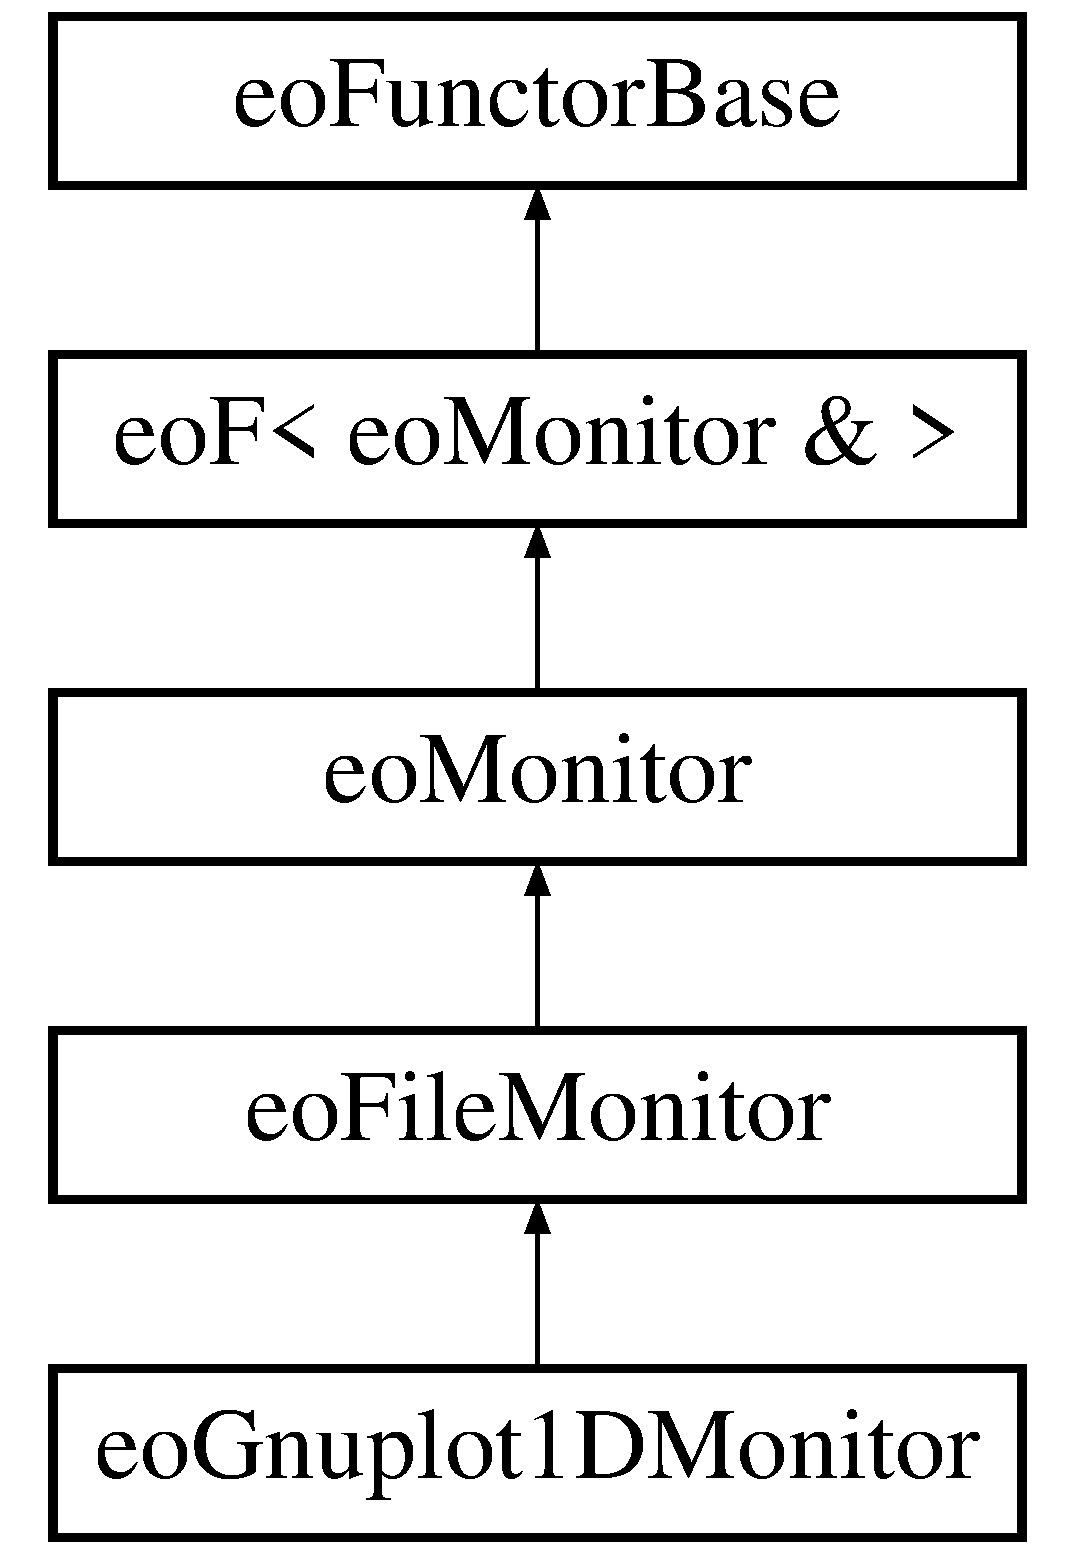
\includegraphics[height=5cm]{classeo_file_monitor}
\end{center}
\end{figure}
\subsection*{Public Member Functions}
\begin{CompactItemize}
\item 
{\bf eo\-File\-Monitor} (std::string \_\-filename, std::string \_\-delim=\char`\"{} \char`\"{}, bool \_\-keep=false, bool \_\-header=false)\label{classeo_file_monitor_a0}

\item 
virtual {\bf eo\-Monitor} \& {\bf operator()} (void)\label{classeo_file_monitor_a1}

\begin{CompactList}\small\item\em The pure virtual function that needs to be implemented by the subclass. \item\end{CompactList}\item 
virtual {\bf eo\-Monitor} \& {\bf operator()} (std::ostream \&os)\label{classeo_file_monitor_a2}

\item 
void {\bf print\-Header} (void)\label{classeo_file_monitor_a3}

\item 
virtual void {\bf print\-Header} (std::ostream \&os)\label{classeo_file_monitor_a4}

\item 
virtual std::string {\bf get\-File\-Name} ()\label{classeo_file_monitor_a5}

\end{CompactItemize}
\subsection*{Private Attributes}
\begin{CompactItemize}
\item 
std::string {\bf filename}\label{classeo_file_monitor_r0}

\item 
std::string {\bf delim}\label{classeo_file_monitor_r1}

\item 
bool {\bf keep}\label{classeo_file_monitor_r2}

\item 
bool {\bf header}\label{classeo_file_monitor_r3}

\item 
bool {\bf firstcall}\label{classeo_file_monitor_r4}

\end{CompactItemize}


\subsection{Detailed Description}
Prints statistics to file. 

Modified the default behavior, so that it erases existing files. Can be modified in the ctor.

\begin{Desc}
\item[Version:]MS 25/11/00 \end{Desc}




Definition at line 44 of file eo\-File\-Monitor.h.

The documentation for this class was generated from the following files:\begin{CompactItemize}
\item 
eo\-File\-Monitor.h\item 
eo\-File\-Monitor.cpp\end{CompactItemize}
